\documentclass[12pt]{article}
\usepackage[utf8]{inputenc}     % 設定字符編碼為 UTF-8
\usepackage{subcaption}         % 支援子圖
\usepackage{fontspec}           % 支持自定義字體
\usepackage{setspace}           % 行距設定
\usepackage{titlesec}           % 標題樣式設定
\usepackage{graphicx}           % 載入插入圖片的包
\usepackage{amsmath}            % 支持數學公式
\usepackage{caption}            % figurename -> 圖
\usepackage{xeCJK}              % 支持 CJK 字體

\usepackage[a4paper,top=2cm,bottom=2cm,left=2cm,right=2cm]{geometry}

\setmainfont{Times New Roman}   % 設定英文主字體(可選)
\setCJKmainfont{DFKai-SB}[
    AutoFakeBold=true,          % 啟用粗體模擬
    AutoFakeSlant=true          % 啟用斜體模擬
]

\onehalfspacing{}               % 設置 1.5 倍行距

% 設定 \section 的字型大小和居中,不顯示節號
\titleformat{\section}[block]
  {\normalfont\fontsize{16}{24}\selectfont\centering}  % 設定字型大小為 16pt,行距為 24pt,並居中顯示
  {}{0em}{}  % 不顯示節號,並設定標題與上方的間距

% 設定 \subsection 與正文字體樣式相同,不顯示節號
\titleformat{\subsection}[block]
  {\normalfont\mdseries\upshape}   % 設定與正文相同的字型樣式
  {}{0em}{}  % 不顯示子節號,並設定標題與上方的間距

% 設定 \subsubsection 與正文字體樣式相同,並加上縮排,不顯示節號
\titleformat{\subsubsection}[block]
  {\normalfont\mdseries\upshape\leftskip=2em}   % 設定與正文相同的字型樣式,並設定左邊縮排 2em
  {}{0em}{}  % 不顯示子子節號,並設定標題與上方的間距

% 設定 \subsubsection 與正文字體樣式相同,並加上縮排,不顯示節號
\titleformat{\subsubsubsection}[block]
  {\normalfont\mdseries\upshape\leftskip=4em}   % 設定與正文相同的字型樣式,並設定左邊縮排 2em
  {}{0em}{}  % 不顯示子子節號,並設定標題與上方的間距

\setlength{\parindent}{2em} % 設定段落的首行縮排為 2em

\renewcommand{\figurename}{圖} % figurename -> 圖

\begin{document}

\section{摘要}

\newpage
\section{壹、前言}

\subsection{一、研究動機}

在高一時,我完成了一個名為「數位鏡面」的專案,靈感源自丹尼爾.羅森(2017)在桃園機場捷運的一系列藝術品。這些作品利用鏡頭捕捉現實畫面,經過電腦計算後,以獨特的方式呈現影像。其中,有一幅作品以線條形式重構畫面,宛如一面極具創意的鏡子(如圖\ref{fig:mirror_example_1}),而我的專案正是以此為藍本進行模仿與實現。

\begin{figure}[htbp]
  \centering
  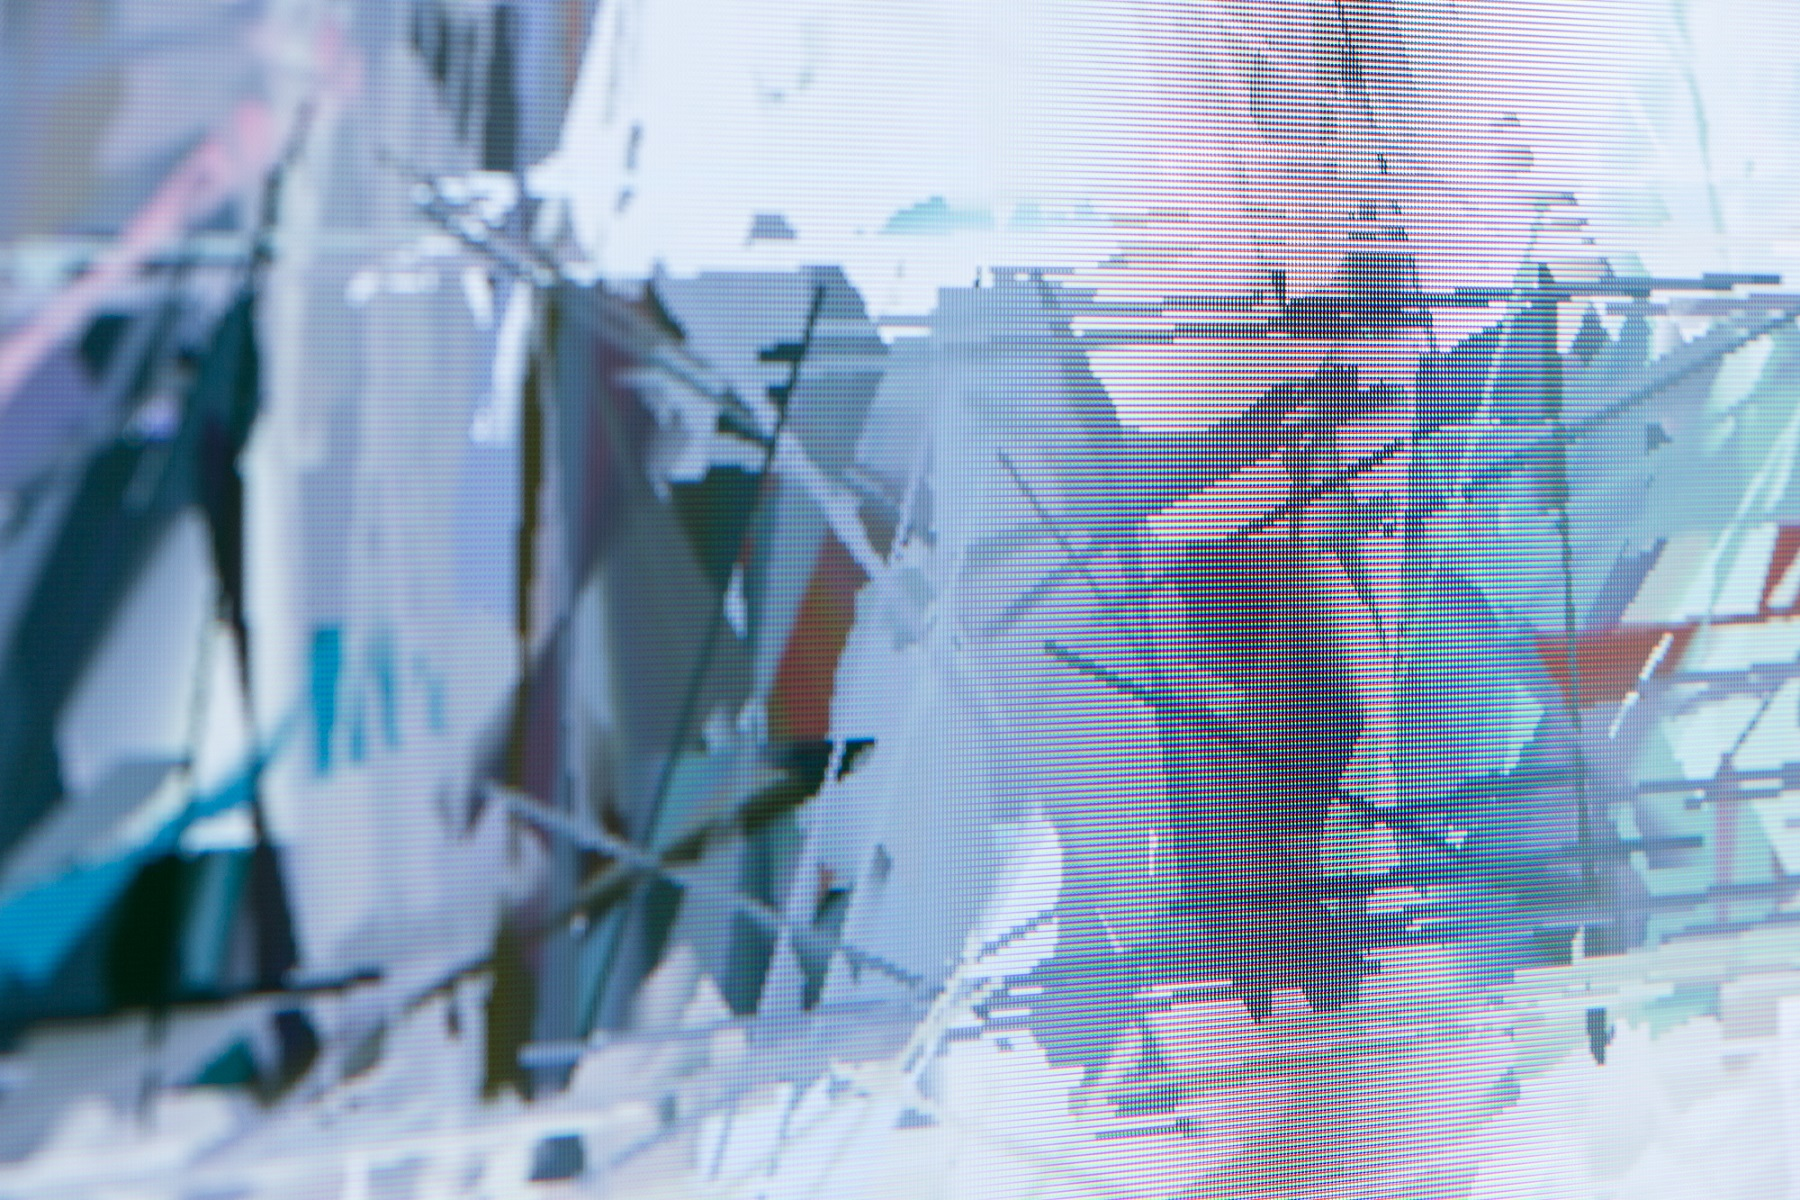
\includegraphics[width=0.8\textwidth]{img//mirror_example_1.jpg}
  \caption{丹尼爾.羅森的數位鏡面}\label{fig:mirror_example_1}
\end{figure}

在實作過程中,我發現許多參數會影響數位鏡面的效果,例如線條的長度與寬度等表層設定,或是每次刷新時繪製的線條數量等底層設定。此外,環境因素的變化也會影響數位鏡面的呈現效果。這些觀察激發了我的好奇心,使我想深入研究各種參數對數位鏡面效果的影響,進一步探索它背後的運作機制。

\subsection{二、研究目的}

\subsubsection{(一)了解不同參數設定對於數位鏡面的影響}
\subsubsection{(二)了解不同影像環境對於數位鏡面的影響}
\subsubsection{(三)探討不同環境與需求下數位鏡面的最優設定}

\newpage

\subsection{三、文獻探討}

\subsubsection{(一)數位鏡面}

數位鏡面最初是丹尼爾·羅森(2017)在機場捷運展示的一系列藝術作品。這些作品透過鏡頭捕捉現實世界的影像,並經由電腦計算處理後,以特殊的方式呈現在螢幕上。影像如圖\ref{fig:mirror_example_23}所示,經過數位化處理後,現實畫面顯得模糊且朦朧,營造出獨特的視覺效果。該系列中的每件作品皆展現了不同的風格與表現形式。本次實驗將聚焦於其中一種以類似線條形式呈現的數位鏡面作品,進行深入探討。

\

\begin{itshape}
  《數位鏡面》由五組鏡面裝置構成,並以攝影機與程式控制觀眾互動與畫面反應機制,透過感應器將臨到作品鏡前的物件或人像,轉化為不同筆觸的動態速寫。
\end{itshape}

\

\begin{figure}[htbp]
  \centering
  % 第一張圖片
  \begin{minipage}[b]{0.45\textwidth}
    \centering
    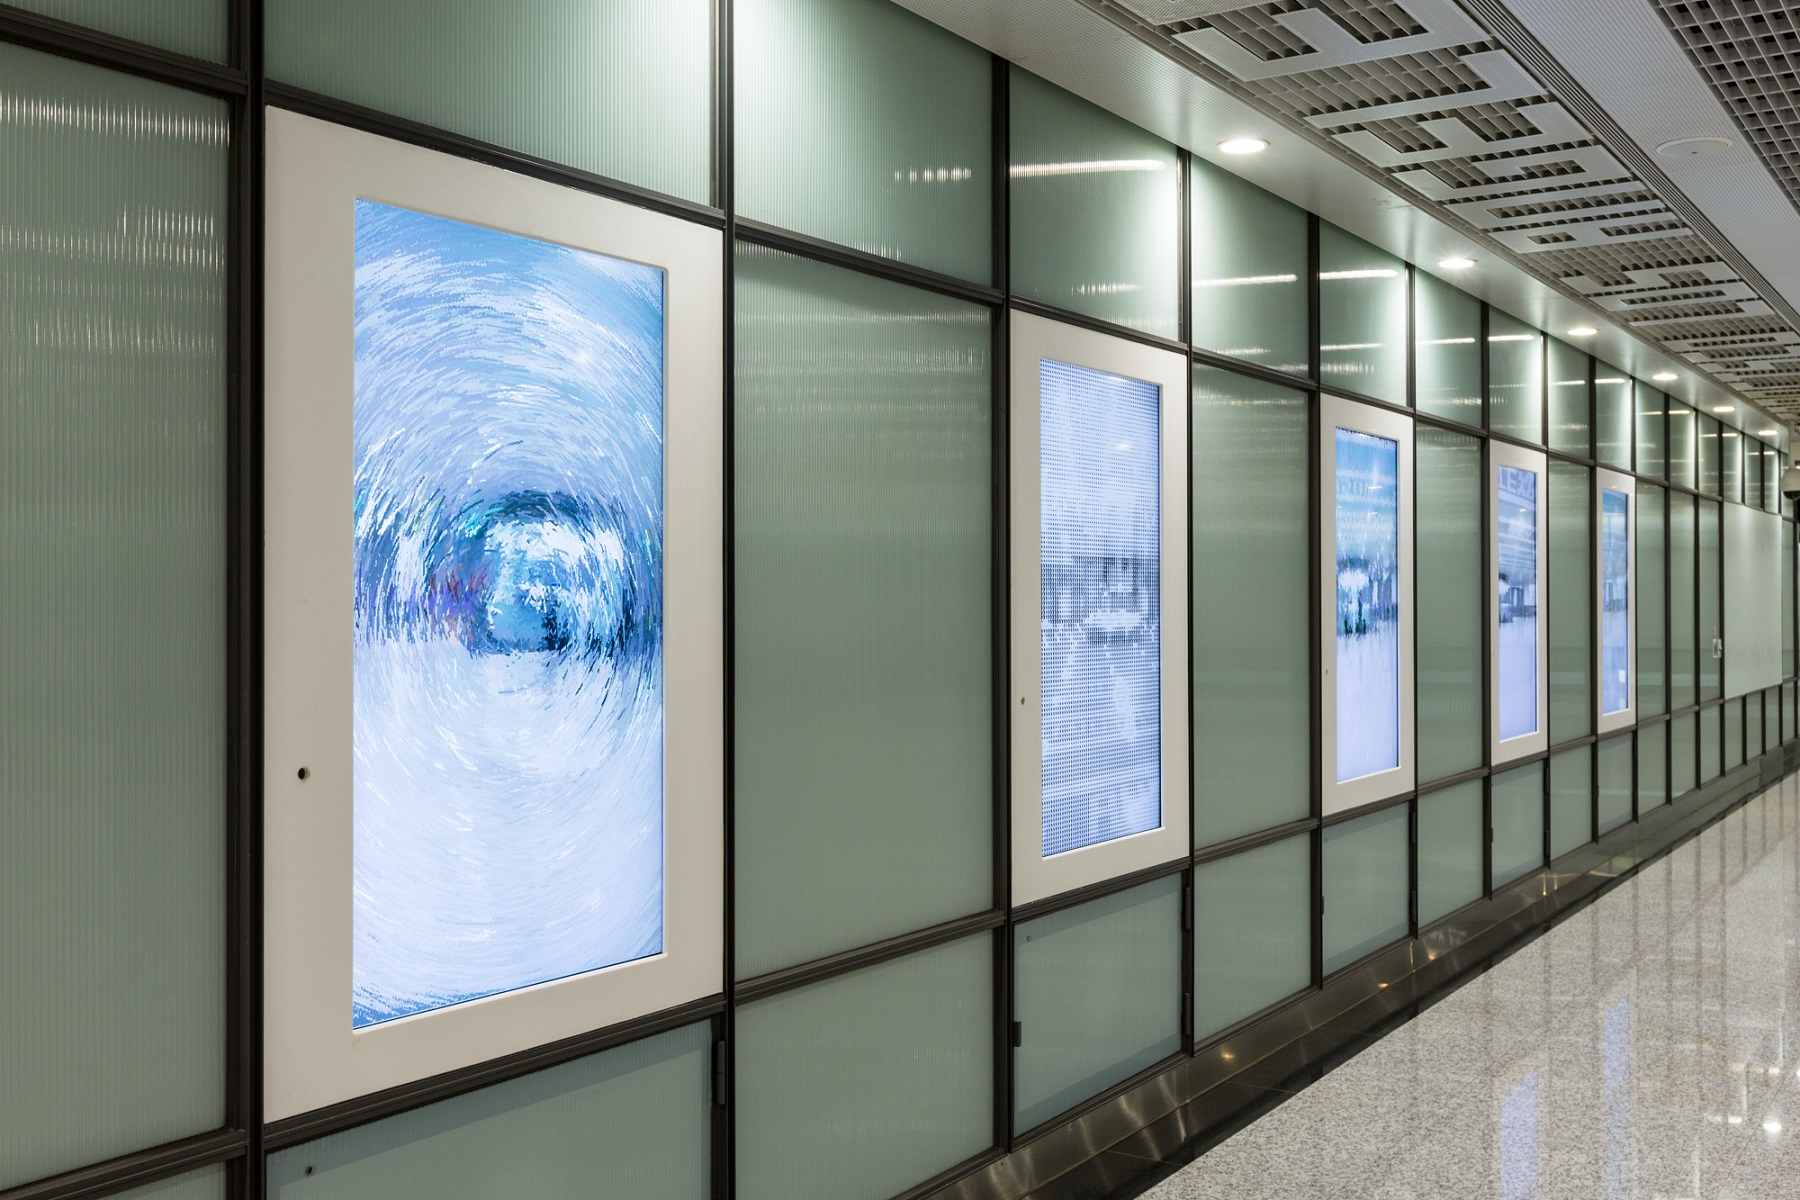
\includegraphics[width=\textwidth]{img/mirror_example_2.jpg}
  \end{minipage}
  \hfill
  % 第二張圖片
  \begin{minipage}[b]{0.45\textwidth}
    \centering
    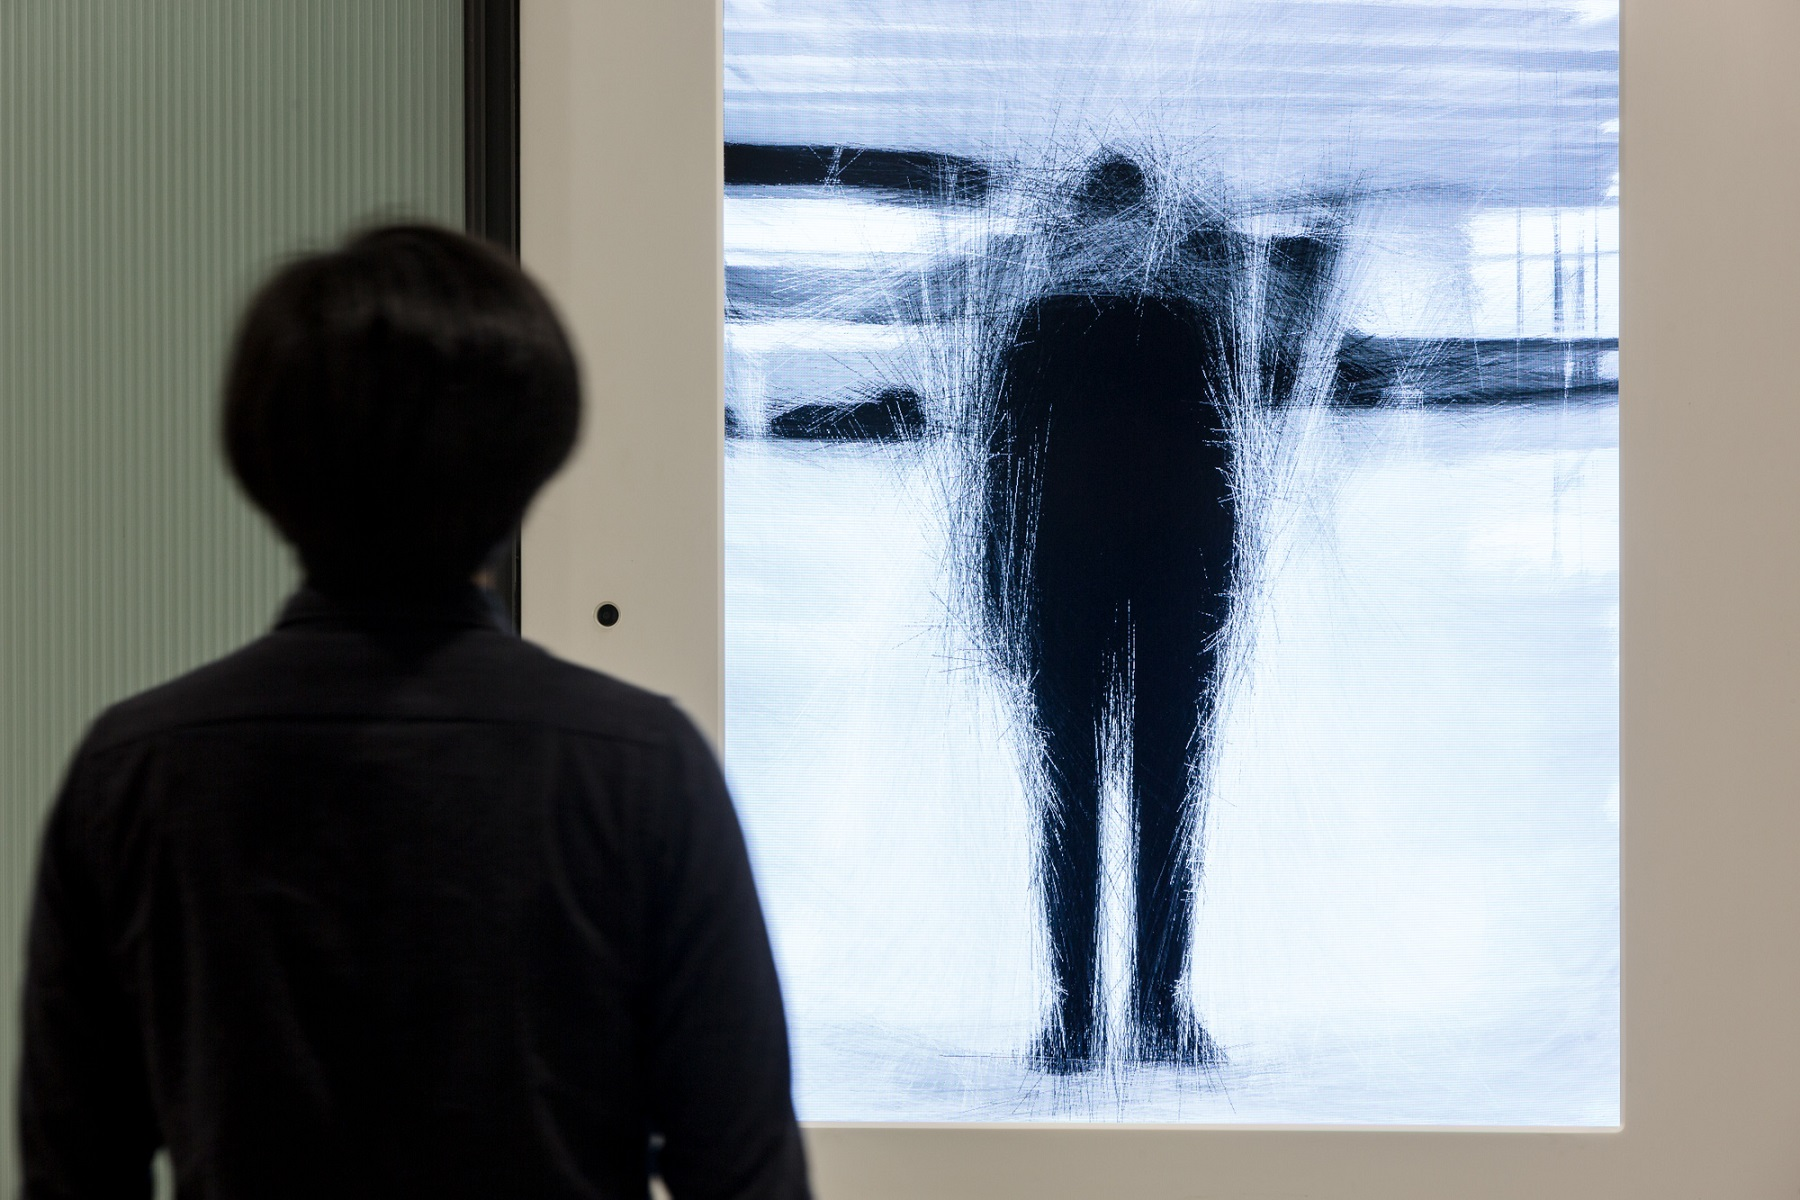
\includegraphics[width=\textwidth]{img/mirror_example_3.jpg}
  \end{minipage}
\caption{丹尼爾.羅森的數位鏡面}\label{fig:mirror_example_23}
\end{figure}

本次研究使用的是 happycorn 在 GitHub 上提供的數位鏡面模仿作品(2024)。程式中展示了以線條為主要呈現方式的數位鏡面,其每一幀的繪製過程包括:讀取影像、繪製多條線條,以及刷新畫面。繪製線條的過程則可細分為以下步驟:模擬一條虛擬線、計算該線條路徑上所有像素點的平均值、以及根據計算結果繪製線條。更詳細的流程如圖所示。

\begin{figure}[htbp]
  \centering
  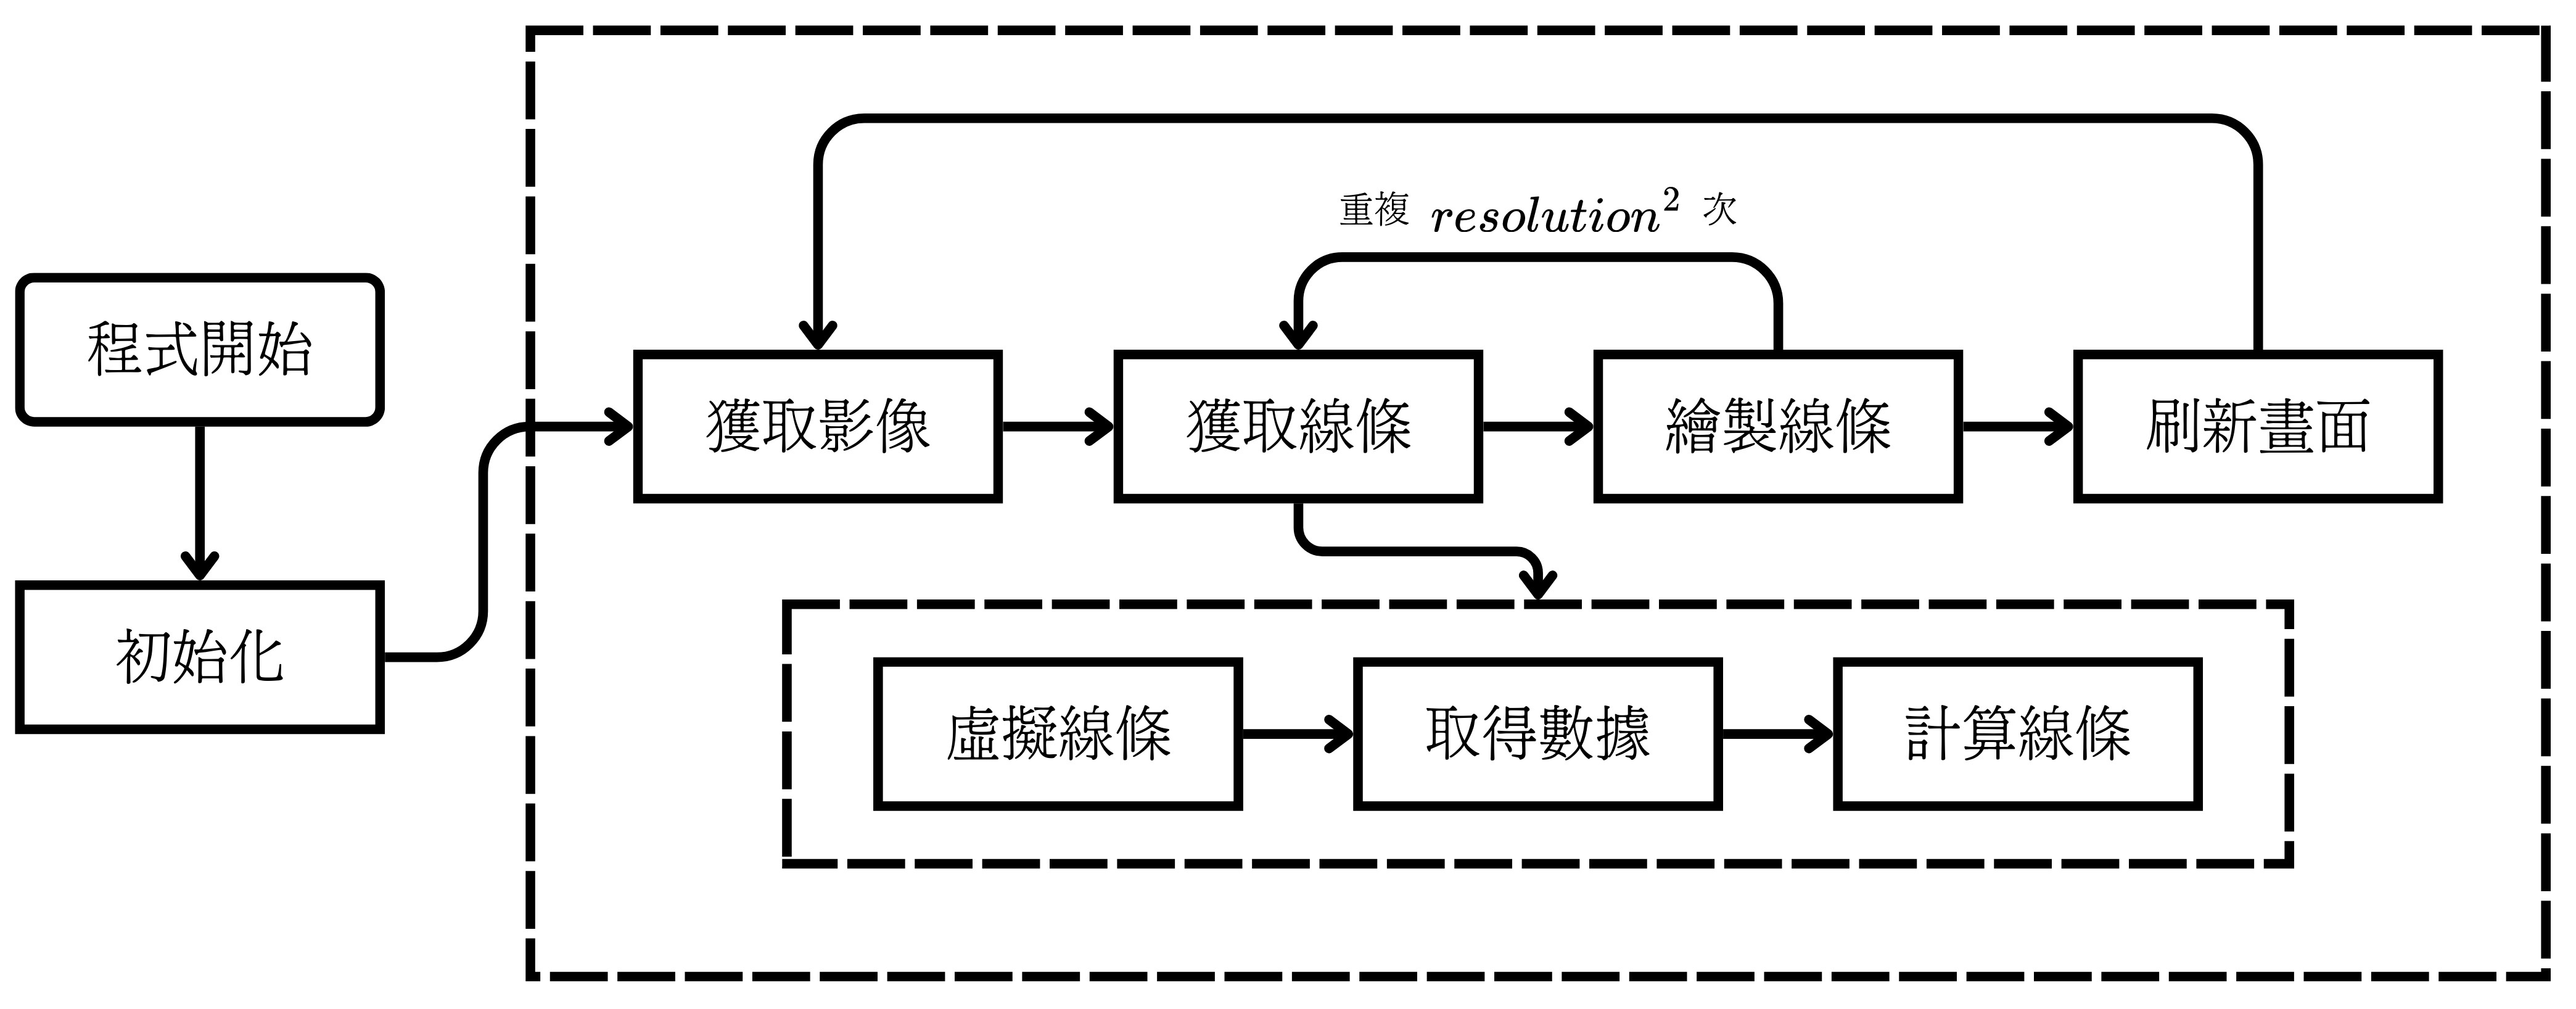
\includegraphics[width=0.8\textwidth]{img//program_flaw.jpg}
  \caption{丹尼爾.羅森的數位鏡面}\label{fig:program_flaw}
\end{figure}

在整面數位鏡面中,可調整的參數有三項:線條寬度(width)、線條長度(length)與解析度(resolution)。線條寬度與長度分別表示數位鏡面在繪製時的線條寬度與長度;而解析度則是與繪製過程中的區域劃分相關。為了同時達成「繪製多條線」與「分散線條位置」的效果,作者透過 for 迴圈將整個鏡面切分為多個小方格,並在每個方格內繪製一條線,解析度即代表這些方格的寬度。

\subsubsection{(二)時間複雜度}

什麼是時間複雜度?

\subsubsection{(三)互動藝術}

數位鏡面等數位藝術究竟在畫什麼?

數位鏡面想要達到怎樣的效果?

\subsubsection{(四)Sum Of Absolute Difference}

照片相似度比較

\newpage
\section{貳、研究設備及器材}

硬體

電腦乙台

軟體

Python、Opencv、Numpy、Plt、Anaconda、Ipynb

\newpage
\section{參、研究過程與方法}

\subsection{一、研究架構圖}

\subsection{二、研究一:數位鏡面的時間複雜度}

\subsubsection{(一)數位鏡面的時間複雜度計算}

\subsubsection{(二)計算結果驗算}

\subsection{三、研究二:數位鏡面輸出結果量化}

\subsubsection{(一)「模糊」的量化}

\subsubsection{(二)「變化」的量化}

\subsection{四、實驗一:各項參數對於數位鏡面的影響}

\subsubsection{(一)線條寬度(width)對於數位鏡面的影響}

\subsubsection{(二)線條長度(lenth)對於數位鏡面的影響}

\subsubsection{(三)解析度(resolution)對於數位鏡面的影響}

\subsection{五、實驗二:不同場景對於數位鏡面的影響}

\subsubsection{(一)背景顏色對於數位鏡面的影響}

顏色差異與顏色數量

\subsubsection{(二)線條長度(lenth)對於數位鏡面的影響}

\subsubsection{(三)解析度(resolution)對於數位鏡面的影響}

\newpage
\section{肆、研究結果}

\subsection{一、研究一:數位鏡面的時間複雜度}

\subsubsection{(一)數位鏡面的時間複雜度計算}

\subsubsection{(二)計算結果驗算}

\subsection{二、研究二:數位鏡面輸出結果量化}

\subsubsection{(一)「模糊」的量化}

\subsubsection{(二)「變化」的量化}

\subsection{三、實驗一:各項參數對於數位鏡面的影響}

\subsubsection{(一)線條寬度(width)對於數位鏡面的影響}

\subsubsection{(二)線條長度(lenth)對於數位鏡面的影響}

\subsubsection{(三)解析度(resolution)對於數位鏡面的影響}

\subsection{四、實驗二:不同場景對於數位鏡面的影響}

\subsubsection{(一)背景顏色對於數位鏡面的影響}

\subsubsection{(二)線條長度(lenth)對於數位鏡面的影響}

\subsubsection{(三)解析度(resolution)對於數位鏡面的影響}

\newpage
\section{伍、討論}

\newpage
\section{陸、結論}

\newpage
\section{柒、參考文獻資料}

https://www.husart.net/?p=372 丹尼爾羅森

https://github.com/happpycorn/Mirror_Line 我的數位鏡面

\end{document}